% vim: ai sw=2 spell spelllang=en

\documentclass[xcolor=dvipsnames,handout]{beamer}

\let\Oldemph\emph
\renewcommand{\emph}[1]{\textcolor{blue}{\Oldemph{#1}}}
\newcommand{\heading}[1]{\textbf{\textcolor{BurntOrange}{#1}}}
\newcommand{\header}[1]{\textbf{\texttt{\textcolor{WildStrawberry}{#1}}}}
\newcommand{\doc}[1]{\textbf{\texttt{\textcolor{OliveGreen}{#1}}}}
\newcommand{\red}[1]{\textcolor{red}{#1}}

\newcommand\kgr{\textsc{kGraft}\xspace}

\mode<presentation>
{
\usetheme{Madrid}
}

\setbeamertemplate{navigation symbols}{}
%\setbeamertemplate{footline}[frame number]{}

\usepackage{adjustbox}
\usepackage[utf8x]{inputenc}
\usepackage{helvet}
\usepackage{mathptmx}
\usepackage[T1]{fontenc}
\usepackage{graphicx}
\usepackage{hyperref}
\usepackage[final]{listings}
\usepackage{multirow}
\usepackage{tikz}
\usepackage[absolute,overlay]{textpos}
\usepackage{xspace}
\usetikzlibrary{arrows, positioning, fit}

\tikzset{tl_state/.style={rounded corners, thick, draw, minimum height=6mm,
	minimum width=12mm, bottom color=black!15, top color=black!5}}
\tikzset{tl_phase/.style={thick, draw, minimum size=8mm}}
\tikzset{tl_edge/.style={<-, >=stealth', semithick}}
\tikzset{invisible/.style={opacity=0},
	visible on/.style={alt={#1{}{invisible}}},
	alt/.code args={<#1>#2#3}{%
          \alt<#1>{\pgfkeysalso{#2}}{\pgfkeysalso{#3}} % \pgfkeysalso doesn't change the path
	},
}
\tikzset{entwid/.style={minimum width=70pt}}
\tikzset{ent/.style={rectangle, rounded corners=4pt, semithick, draw, inner sep=5pt, minimum height=80pt, entwid}}
\tikzset{fillbot/.style={fill=lightgray, rectangle, entwid, minimum height=10pt}}
\tikzset{filltop/.style={fillbot, rounded corners=4pt, minimum height=15pt}}
\tikzset{codearrow/.style={->, shorten >= 10pt, >=stealth', semithick, dotted}}
\tikzset{insnode/.style={fill=lightgray, rectangle, semithick, draw}}
\tikzset{connarr/.style={semithick, ->, shorten >= 4pt, shorten <= 4pt}}

\pgfdeclarelayer{background}
\pgfsetlayers{background,main}

\lstset{tabsize=2,numbers=none,showstringspaces=false,breaklines=true,
	breakatwhitespace=true,escapeinside={(*@}{@*)},
	basicstyle=\scriptsize,keywordstyle=\bfseries\color{OliveGreen},
	commentstyle=\color{blue}, columns=flexible, language=C,
	morekeywords={asm}}

\newcommand{\cmd}[2][]{\lstinline[columns=fullflexible, language=bash,
	basicstyle=\ttfamily, #1]$#2$}
\newcommand{\code}[2][]{\lstinline[columns=fullflexible, basicstyle=\ttfamily,
	#1]$#2$}

\definecolor{mygray}{gray}{.9}

\title{kGraft}
\subtitle{Live patching of the Linux kernel}
\date[September 25\textsuperscript{th} 2014, Paris]{September
25\textsuperscript{th} 2014 \\ Paris, France}

\author[Jiri~Slaby]{Jiří Kosina, Petr Mládek, Vojtěch Pavlík, \textbf{Jiri~Slaby}}

\institute{SUSE Labs}

\titlegraphic{\flushright
\includegraphics[width=.25\textwidth]{suse_logo_w-tag_pantone}~~~~~}

\begin{document}

\begin{frame}
  \titlepage
\end{frame}

%%%%%%%%%%%%%%%%%%%%%%%

\begin{frame}
  \frametitle{Why Live Patching?}

  \begin{itemize}
    \item 1000 machines \& severe security problem
    \begin{itemize}
      \item Needs fixing \emph{now}!
    \end{itemize}

    \pause

    \item Rebooting the machines
    \begin{itemize}
      \item Is not a quick way to fix an issue
      \item Has a risk of not coming up
    \end{itemize}

    \pause

    \item \emph{Live patching}
    \begin{itemize}
      \item Allows quick response
      \item Leaves an actual update to a scheduled downtime window
    \end{itemize}

  \end{itemize}

\end{frame}

\begin{frame}
  \frametitle{Where is Live Patching Useful?}

  \begin{itemize}
    \item Common tiers of change management
    \begin{enumerate}
      \item Incident response -- we are exploited
      \item Emergency change -- we could be exploited (we are vulnerable)
      \item Scheduled change -- time is not critical, we are safe
    \end{enumerate}

    \pause

    \item Live patching fits in with 1 and 2

  \end{itemize}

\end{frame}

\begin{frame}
  \frametitle{Presentation Outline}

  \tableofcontents

\end{frame}

\section{\kgr}
\frame{\sectionpage}

\begin{frame}
  \frametitle{\kgr}

  \begin{itemize}
    \item Research project
    \item Live patching technology
    \item Developed by SUSE Labs
    \item Specifically for the Linux kernel

    \pause

    \item Based on modern Linux technologies
    \begin{itemize}
      \item INT3/IPI-NMI self-modifying code
      \item Lazy update mechanism
      \item \code{fentry}-based NOP space allocation
      \item Standard kernel module loading/linking mechanisms
    \end{itemize}

  \end{itemize}

\end{frame}

\begin{frame}
  \frametitle{Advantages of \kgr}

  \begin{itemize}
    \item Does not require stopping the kernel
    \pause
    \begin{itemize}
      \item Ever!
      \pause
      \item Not even for short time periods
      \item Unlike competing technologies
    \end{itemize}

    \pause

    \item Allows code review on \kgr patch sources
    \begin{itemize}
      \item Patches can be built from C source directly
      \item No need for object code manipulation
      \begin{itemize}
	\item Only an alternative: object code based automated patch generation
      \end{itemize}
    \end{itemize}

    \pause

    \item kGraft is lean
    \begin{itemize}
      \item Small amount of code
      \item Leveraging other Linux technologies
      \item No complex instruction en/decoders or such
    \end{itemize}

  \end{itemize}

\end{frame}

\begin{frame}
  \frametitle{How does \kgr work?}

  \begin{itemize}
    \item A kGraft patch is a \cmd{.ko} kernel module
    \item The \cmd{.ko} is inserted into the kernel using \cmd{insmod}
    \begin{itemize}
      \item All linking (incl.\ the fix) is done by kernel
    \end{itemize}

    \pause

    \item \kgr replaces whole functions in the kernel
    \begin{itemize}
      \item Even while those functions may be executed
    \end{itemize}

    \pause

    \item An updated \kgr module can \emph{replace} an existing patch
  \end{itemize}

\end{frame}

\begin{frame}
  \frametitle{Limitations}

  \begin{itemize}
    \item kGraft is designed for fixing critical bugs
    \begin{itemize}
      \item Primarily for simple changes
    \end{itemize}

    \pause

    \item Changes in kernel data structure layout require special care
    \begin{itemize}
      \item Depending on the size of the change, reboot may be needed
      \item Same as with other live patching techniques
    \end{itemize}

    \pause

    \item \kgr depends on a stable build environment
    \begin{itemize}
      \item Having history of built kernels
      \item Best suited for
      \begin{itemize}
	\item Linux distributions
	\item Their customers
	\item Anyone who builds their own kernels
      \end{itemize}
      \item Not good for 3rd party support 
    \end{itemize}
  \end{itemize}

\end{frame}

\section{\kgr Internals}
\frame{\sectionpage}

\begin{frame}
  \frametitle{\kgr and \code{fentry}}

  \begin{itemize}
    \item \kgr needs some space at the start of a function
    \begin{itemize}
      \item To insert a jump to a patched function
    \end{itemize}

    \pause

    \item The space can be provided by \textsc{Gcc} profiling
    \begin{itemize}
      \item \cmd{-pg -mfentry}
      \item \kgr uses this
    \end{itemize}

    \begin{uncoverenv}<3->
    \item \code{fentry} call instructions
    \begin{itemize}
      \item Patched out at boot
      \item Replaced with 5-byte NOPs
    \end{itemize}
    \end{uncoverenv}

  \end{itemize}

  \begin{center}
    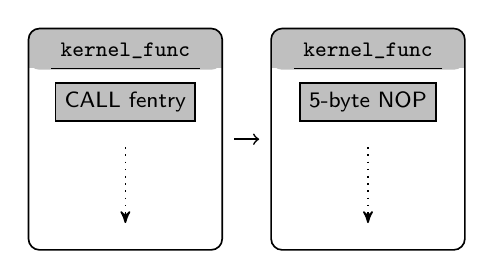
\begin{tikzpicture}[node distance=6mm, font=\sffamily\footnotesize]
      %%%%%%%%%%%%%% 1
      \node [visible on=<2->, ent] (WHOLE1) {};

      \node [visible on=<2->] (FNAME1) [below=2pt of WHOLE1.north] {\code{kernel_func}};
      \path [visible on=<2->, semithick] (FNAME1.south east) edge (FNAME1.south west);
      \begin{pgfonlayer}{background}
	\node [visible on=<2->, filltop] (TOPGRa1) [below=0pt of WHOLE1.north] {};
	\node [visible on=<2->, fillbot] (TOPGRb1) [above=0pt of FNAME1.south] {};
      \end{pgfonlayer}

      \node [visible on=<2->, insnode] (INSN1) [below=5pt of FNAME1] { CALL fentry };

      \node (ARROW_START1) [below=2pt of INSN1] {}
	edge[visible on=<2->, codearrow] node {} (WHOLE1.south);

      %%%%%%%%%%%%%% 2
      \node [visible on=<3->, ent] (WHOLE2) [right=of WHOLE1] {};

      \node [visible on=<3->] (FNAME2) [below=2pt of WHOLE2.north] {\code{kernel_func}};
      \path [visible on=<3->, semithick] (FNAME2.south east) edge (FNAME2.south west);
      \begin{pgfonlayer}{background}
	\node [visible on=<3->, filltop] (TOPGRa2) [below=0pt of WHOLE2.north] {};
	\node [visible on=<3->, fillbot] (TOPGRb2) [above=0pt of FNAME2.south] {};
      \end{pgfonlayer}

      \node [visible on=<3->, insnode] (INSN2) [below=5pt of FNAME2] { 5-byte NOP };

      \node (ARROW_START2) [below=2pt of INSN2] {}
	edge[visible on=<3->, codearrow] node {} (WHOLE2.south);

      %%%%%%%%%%%%%% arrows
      \path [visible on=<3->, connarr] (WHOLE1) edge (WHOLE2);

    \end{tikzpicture}
  \end{center}

\end{frame}

\begin{frame}[fragile]
  \frametitle{Using 5-byte NOPs Space}

  \heading{\kgr uses the ftrace infrastructure to perform patching}\\
  INT3 handler is installed with a JMP to the destination address

  \begin{enumerate}
    \item<2-> First byte of NOP is replaced by INT3
    \item<3-> Remaining bytes are replaced by address
    \item<4-> First byte is replaced by JMP
    \item<5-> NMI IPIs are used to flush instruction decoders on other CPUs
  \end{enumerate}

  \begin{center}
    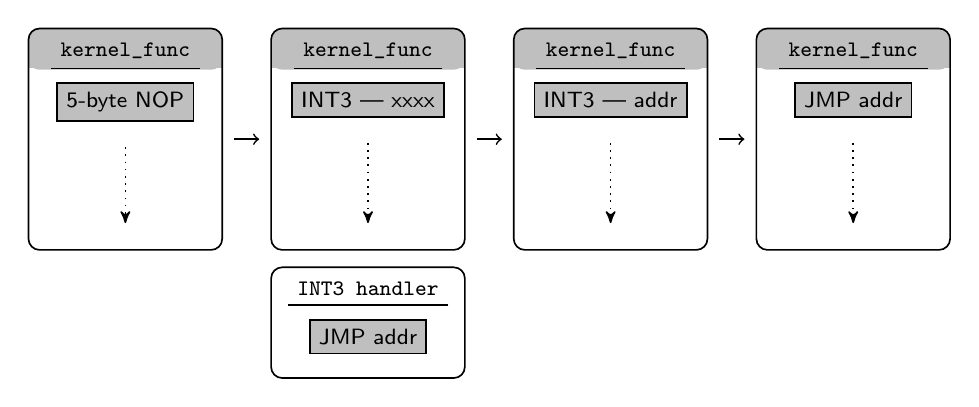
\begin{tikzpicture}[node distance=6mm, font=\sffamily\footnotesize]
      %%%%%%%%%%%%%% 1
      \node [visible on=<1->, ent] (WHOLE1) {};

      \node [visible on=<1->] (FNAME1) [below=2pt of WHOLE1.north] {\code{kernel_func}};
      \path [visible on=<1->, semithick] (FNAME1.south east) edge (FNAME1.south west);
      \begin{pgfonlayer}{background}
	\node [visible on=<1->, filltop] (TOPGRa1) [below=0pt of WHOLE1.north] {};
	\node [visible on=<1->, fillbot] (TOPGRb1) [above=0pt of FNAME1.south] {};
      \end{pgfonlayer}

      \node [visible on=<1->, insnode] (INSN1) [below=5pt of FNAME1] { 5-byte NOP };

      \node (ARROW_START1) [below=2pt of INSN1] {}
	edge[visible on=<1->, codearrow] node {} (WHOLE1.south);

      %%%%%%%%%%%%%% 2
      \node [visible on=<2->, ent] (WHOLE2) [right=of WHOLE1] {};

      \node [visible on=<2->] (FNAME2) [below=2pt of WHOLE2.north] {\code{kernel_func}};
      \path [visible on=<2->, semithick] (FNAME2.south east) edge (FNAME2.south west);
      \begin{pgfonlayer}{background}
	\node [visible on=<2->, filltop] (TOPGRa2) [below=0pt of WHOLE2.north] {};
	\node [visible on=<2->, fillbot] (TOPGRb2) [above=0pt of FNAME2.south] {};
      \end{pgfonlayer}

      \node [visible on=<2->, insnode] (INSN2) [below=5pt of FNAME2] { INT3 | xxxx };

      \node (ARROW_START2) [below=2pt of INSN2] {}
	edge[visible on=<2->, codearrow] node {} (WHOLE2.south);

      %%%%%%%%%%%%%% INT3 handler
      \node [visible on=<2->, ent, minimum height=40pt] (WHOLEINT3) [below=2mm of WHOLE2] {};

      \node [visible on=<2->] (FNAMEINT3) [below=2pt of WHOLEINT3.north] {\code{INT3 handler}};
      \path [visible on=<2->, semithick] (FNAMEINT3.south east) edge (FNAMEINT3.south west);
%      \begin{pgfonlayer}{background}
%	\node [visible on=<2->, filltop] (TOPGRa2) [below=0pt of WHOLE2.north] {};
%	\node [visible on=<2->, fillbot] (TOPGRb2) [above=0pt of FNAME2.south] {};
%      \end{pgfonlayer}

      \node [visible on=<2->, insnode] (INSNINT3) [below=5pt of FNAMEINT3] { JMP addr };

      %%%%%%%%%%%%%% 3
      \node [visible on=<3->, ent] (WHOLE3) [right=of WHOLE2] {};

      \node [visible on=<3->] (FNAME3) [below=2pt of WHOLE3.north] {\code{kernel_func}};
      \path [visible on=<3->, semithick] (FNAME3.south east) edge (FNAME3.south west);
      \begin{pgfonlayer}{background}
	\node [visible on=<3->, filltop] (TOPGRa3) [below=0pt of WHOLE3.north] {};
	\node [visible on=<3->, fillbot] (TOPGRb3) [above=0pt of FNAME3.south] {};
      \end{pgfonlayer}

      \node [visible on=<3->, insnode] (INSN3) [below=5pt of FNAME3] { INT3 | addr };

      \node (ARROW_START3) [below=2pt of INSN3] {}
	edge[visible on=<3->, codearrow] node {} (WHOLE3.south);

      %%%%%%%%%%%%%% 4
      \node [visible on=<4->, ent] (WHOLE4) [right=of WHOLE3] {};

      \node [visible on=<4->] (FNAME4) [below=2pt of WHOLE4.north] {\code{kernel_func}};
      \path [visible on=<4->, semithick] (FNAME4.south east) edge (FNAME4.south west);
      \begin{pgfonlayer}{background}
	\node [visible on=<4->, filltop] (TOPGRa4) [below=0pt of WHOLE4.north] {};
	\node [visible on=<4->, fillbot] (TOPGRb4) [above=0pt of FNAME4.south] {};
      \end{pgfonlayer}

      \node [visible on=<4->, insnode] (INSN4) [below=5pt of FNAME4] { JMP addr };

      \node (ARROW_START4) [below=2pt of INSN4] {}
	edge[visible on=<4->, codearrow] node {} (WHOLE4.south);

      %%%%%%%%%%%%%% arrows
      \path [visible on=<2->, connarr] (WHOLE1) edge (WHOLE2);
      \path [visible on=<3->, connarr] (WHOLE2) edge (WHOLE3);
      \path [visible on=<4->, connarr] (WHOLE3) edge (WHOLE4);

    \end{tikzpicture}
  \end{center}

\end{frame}

\begin{frame}
  \frametitle{Patching a Function}

  \begin{itemize}
    \item Patching during runtime, no \code{stop_kernel();}

    \pause

    \item Callers are never patched
    \begin{itemize}
      \item Rather, callee's NOPs are replaced by a JMP to the new function
      \item JMP remains forever
    \end{itemize}

    \pause
    \bigskip

    \item But this takes care of function pointers, including in structures
    \begin{itemize}
      \item Like indirect calls (\code{handler->function()})
    \end{itemize}

    \pause

    \item Does not require saving any old data in case we want to un-patch
  \end{itemize}

\end{frame}

\begin{frame}
  \frametitle{Patching a Function in Pictures}

  \begin{center}
    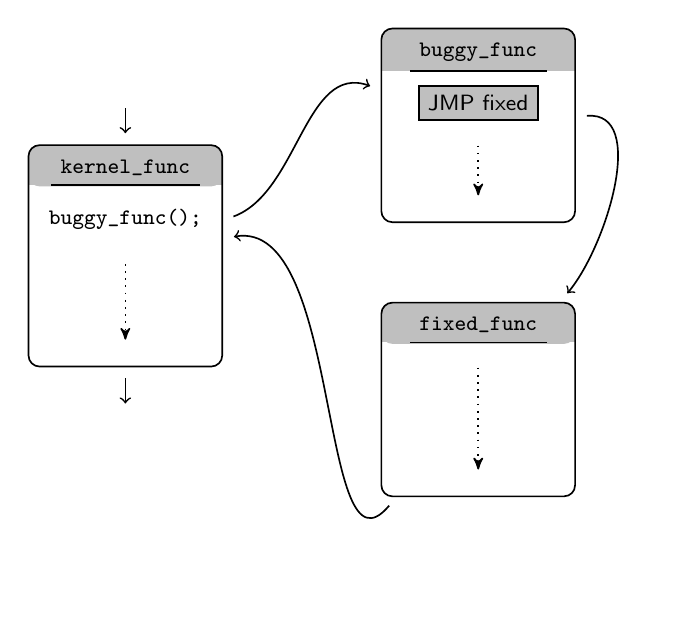
\begin{tikzpicture}[node distance=6mm, font=\sffamily\footnotesize]
      %%%%%%%%%%%%%% 1
      \node [visible on=<1->, ent] (WHOLE1) {};

      \node [visible on=<1->] (FNAME1) [below=2pt of WHOLE1.north] {\code{kernel_func}};
      \path [visible on=<1->, semithick] (FNAME1.south east) edge (FNAME1.south west);
      \begin{pgfonlayer}{background}
	\node [visible on=<1->, filltop] (TOPGRa1) [below=0pt of WHOLE1.north] {};
	\node [visible on=<1->, fillbot] (TOPGRb1) [above=0pt of FNAME1.south] {};
      \end{pgfonlayer}

      \node [visible on=<1->] (INSN1) [below=5pt of FNAME1] { \code{buggy_func();} };

      \node (ARROW_START1) [below=2pt of INSN1] {}
	edge[visible on=<1->, codearrow] node {} (WHOLE1.south);

      %%%%%%%%%%%%%% 2
      \node [visible on=<2->, ent, minimum height=70pt] (WHOLE2) [above right= -1cm and 2cm of WHOLE1] {};

      \node [visible on=<2->] (FNAME2) [below=2pt of WHOLE2.north] {\code{buggy_func}};
      \path [visible on=<2->, semithick] (FNAME2.south east) edge (FNAME2.south west);
      \begin{pgfonlayer}{background}
	\node [visible on=<2->, filltop] (TOPGRa2) [below=0pt of WHOLE2.north] {};
	\node [visible on=<2->, fillbot] (TOPGRb2) [above=0pt of FNAME2.south] {};
      \end{pgfonlayer}

      \node [visible on=<2->, insnode] (INSN2) [below=5pt of FNAME2] { JMP fixed };

      \node (ARROW_START2) [below=2pt of INSN2] {}
	edge[visible on=<2->, codearrow] node {} (WHOLE2.south);

      %%%%%%%%%%%%%% 3
      \node [visible on=<3->, ent, minimum height=70pt] (WHOLE3) [below=1cm of WHOLE2] {};

      \node [visible on=<3->] (FNAME3) [below=2pt of WHOLE3.north] {\code{fixed_func}};
      \path [visible on=<3->, semithick] (FNAME3.south east) edge (FNAME3.south west);
      \begin{pgfonlayer}{background}
	\node [visible on=<3->, filltop] (TOPGRa3) [below=0pt of WHOLE3.north] {};
	\node [visible on=<3->, fillbot] (TOPGRb3) [above=0pt of FNAME3.south] {};
      \end{pgfonlayer}

      \node (ARROW_START3) [below=2pt of FNAME3] {}
	edge[visible on=<3->, codearrow] node {} (WHOLE3.south);

      %%%%%%%%%%%%%% arrows
      \path [visible on=<2->, connarr, out=20, in = 160] (WHOLE1) edge (WHOLE2);
      \path [visible on=<3->, connarr, out=5, in = 50] (WHOLE2) edge (WHOLE3);
      \path [visible on=<3->, connarr, out= 230, in = 10] (WHOLE3) edge (WHOLE1);

      \node (WHOLE1top) [above=of WHOLE1] {}
	edge[connarr] node {} (WHOLE1);
      \node (WHOLE1bot) [below=of WHOLE1] {}
	edge[connarr, <-] node {} (WHOLE1);

    \end{tikzpicture}
  \end{center}

\end{frame}

\begin{frame}
  \frametitle{Issue: Non-consistency}

  \heading{What happens when}
  \begin{itemize}
    \item Replaced function changes semantics and subsequent calls rely on each other?
    \item It is called recursively?
  \end{itemize}

  \begin{center}
    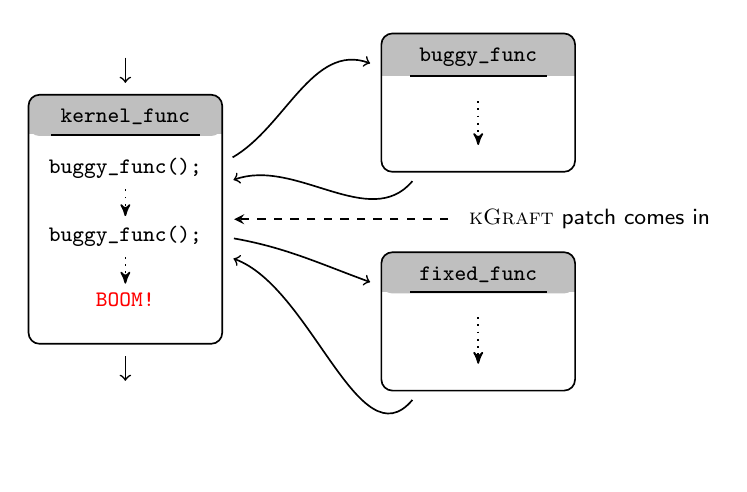
\begin{tikzpicture}[node distance=6mm, font=\sffamily\footnotesize]
      %%%%%%%%%%%%%% 1
      \node [visible on=<1->, ent, minimum height=90pt] (WHOLE1) {};

      \node [visible on=<1->] (FNAME1) [below=2pt of WHOLE1.north] {\code{kernel_func}};
      \path [visible on=<1->, semithick] (FNAME1.south east) edge (FNAME1.south west);
      \begin{pgfonlayer}{background}
	\node [visible on=<1->, filltop] (TOPGRa1) [below=0pt of WHOLE1.north] {};
	\node [visible on=<1->, fillbot] (TOPGRb1) [above=0pt of FNAME1.south] {};
      \end{pgfonlayer}

      \node [visible on=<1->] (INSNa1) [below=5pt of FNAME1] { \code{buggy_func();} };

      \node [visible on=<1->] (INSNb1) [below=10pt of INSNa1] { \code{buggy_func();} }
        edge[visible on=<1->, codearrow, <-, shorten < = 0pt, shorten > = 0pt] node {} (INSNa1);

      \node [visible on=<5->] (INSNc1) [below=10pt of INSNb1] { \textcolor{red}{\code{BOOM!}} }
        edge[visible on=<1->, codearrow, <-, shorten < = 0pt, shorten > = 0pt] node {} (INSNb1);

      %%%%%%%%%%%%%% 2
      \node [visible on=<2->, ent, minimum height=50pt] (WHOLE2) [above right= -1cm and 2cm of WHOLE1] {};

      \node [visible on=<2->] (FNAME2) [below=2pt of WHOLE2.north] {\code{buggy_func}};
      \path [visible on=<2->, semithick] (FNAME2.south east) edge (FNAME2.south west);
      \begin{pgfonlayer}{background}
	\node [visible on=<2->, filltop] (TOPGRa2) [below=0pt of WHOLE2.north] {};
	\node [visible on=<2->, fillbot] (TOPGRb2) [above=0pt of FNAME2.south] {};
      \end{pgfonlayer}

      \node (ARROW_START2) [below=2pt of FNAME2] {}
	edge[visible on=<2->, codearrow] node {} (WHOLE2.south);

      %%%%%%%%%%%%%% 3
      \node [visible on=<4->, ent, minimum height=50pt] (WHOLE3) [below=1cm of WHOLE2] {};

      \node [visible on=<4->] (FNAME3) [below=2pt of WHOLE3.north] {\code{fixed_func}};
      \path [visible on=<4->, semithick] (FNAME3.south east) edge (FNAME3.south west);
      \begin{pgfonlayer}{background}
	\node [visible on=<4->, filltop] (TOPGRa3) [below=0pt of WHOLE3.north] {};
	\node [visible on=<4->, fillbot] (TOPGRb3) [above=0pt of FNAME3.south] {};
      \end{pgfonlayer}

      \node (ARROW_START3) [below=2pt of FNAME3] {}
	edge[visible on=<4->, codearrow] node {} (WHOLE3.south);

      %%%%%%%%%%%%%% kgr
      \node (KGRCOMES) [visible on=<3->, right=3cm of WHOLE1] {\kgr patch comes in}
        edge[visible on=<3->, connarr, dashed, >=stealth] node {} (WHOLE1.east);

      %%%%%%%%%%%%%% arrows
      \path [visible on=<2->, connarr, out=30, in = 160] (WHOLE1) edge (WHOLE2);
      \path [visible on=<2->, connarr, out=230, in = 20] (WHOLE2) edge (WHOLE1);
      \path [visible on=<4->, connarr, out=350, in = 160] (WHOLE1) edge (WHOLE3);
      \path [visible on=<4->, connarr, out=230, in = 340] (WHOLE3) edge (WHOLE1);

      \node (WHOLE1top) [above=of WHOLE1] {}
	edge[connarr] node {} (WHOLE1);
      \node (WHOLE1bot) [below=of WHOLE1] {}
	edge[connarr, <-] node {} (WHOLE1);

    \end{tikzpicture}
  \end{center}

\end{frame}

\begin{frame}
  \frametitle{Cure: RCU-like Replacement}

  \begin{itemize}
    \item We need to provide a consistent ``world-view'' to each thread
    \begin{itemize}
      \item User processes
      \item Kernel processes
      \item Interrupts
    \end{itemize}

    \pause

    \item Solution: ``reality check'' trampoline
    \begin{itemize}
      \item Per-thread flag set on each kernel entry/exit
    \end{itemize}

  \end{itemize}

\end{frame}

\begin{frame}
  \frametitle{RCU-like Replacement}

  \begin{center}
    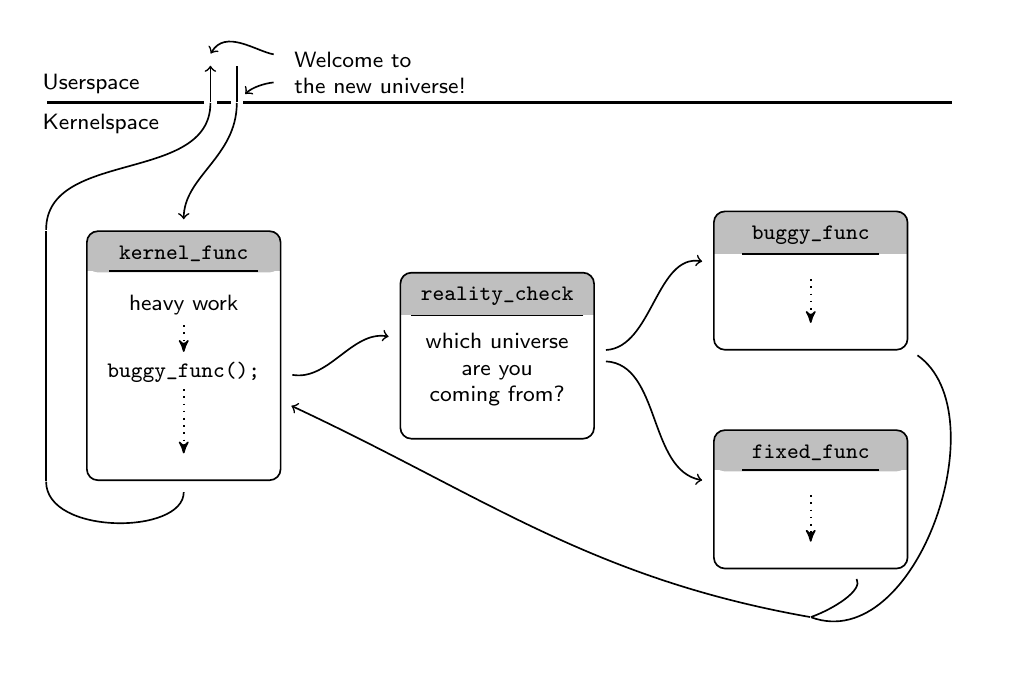
\begin{tikzpicture}[node distance=6mm, font=\sffamily\footnotesize]
      %%%%%%%%%%%%%% kern_fun
      \node [visible on=<1->, ent, minimum height=90pt] (WHOLE1) {};

      \node [visible on=<1->] (FNAME1) [below=2pt of WHOLE1.north] {\code{kernel_func}};
      \path [visible on=<1->, semithick] (FNAME1.south east) edge (FNAME1.south west);
      \begin{pgfonlayer}{background}
	\node [visible on=<1->, filltop] (TOPGRa1) [below=0pt of WHOLE1.north] {};
	\node [visible on=<1->, fillbot] (TOPGRb1) [above=0pt of FNAME1.south] {};
      \end{pgfonlayer}

      \node [visible on=<1->] (INSNa1) [below=5pt of FNAME1] { heavy work };

      \node [visible on=<1->] (INSNb1) [below=10pt of INSNa1] { \code{buggy_func();} }
        edge[visible on=<1->, codearrow, <-, shorten < = 0pt, shorten > = 0pt] node {} (INSNa1);

      \node (ARROW_START1) [below=-8pt of INSNb1] {}
	edge[visible on=<1->, codearrow, shorten < = 0pt] node {} (WHOLE1.south);

      %%%%%%%%%%%%%% reality
      \node [visible on=<2->, ent, minimum height=60pt] (WHOLER) [right= 1.5cm of WHOLE1] {};

      \node [visible on=<2->] (FNAMER) [below=2pt of WHOLER.north] {\code{reality_check}};
      \path [visible on=<2->, semithick] (FNAMER.south east) edge (FNAMER.south west);
      \begin{pgfonlayer}{background}
	\node [visible on=<2->, filltop] (TOPGRaR) [below=0pt of WHOLER.north] {};
	\node [visible on=<2->, fillbot] (TOPGRbR) [above=0pt of FNAMER.south] {};
      \end{pgfonlayer}

      \node [visible on=<2->] (INSN2) [below=3pt of FNAMER, align=center] { which universe \\ are you \\ coming from? };

      %%%%%%%%%%%%%% buggy
      \node [visible on=<3->, ent, minimum height=50pt] (WHOLE2) [above right= -1cm and 1.5cm of WHOLER] {};

      \node [visible on=<3->] (FNAME2) [below=2pt of WHOLE2.north] {\code{buggy_func}};
      \path [visible on=<3->, semithick] (FNAME2.south east) edge (FNAME2.south west);
      \begin{pgfonlayer}{background}
	\node [visible on=<3->, filltop] (TOPGRa2) [below=0pt of WHOLE2.north] {};
	\node [visible on=<3->, fillbot] (TOPGRb2) [above=0pt of FNAME2.south] {};
      \end{pgfonlayer}

      \node (ARROW_START2) [below=2pt of FNAME2] {}
	edge[visible on=<3->, codearrow] node {} (WHOLE2.south);

      %%%%%%%%%%%%%% fixed
      \node [visible on=<3->, ent, minimum height=50pt] (WHOLE3) [below=1cm of WHOLE2] {};

      \node [visible on=<3->] (FNAME3) [below=2pt of WHOLE3.north] {\code{fixed_func}};
      \path [visible on=<3->, semithick] (FNAME3.south east) edge (FNAME3.south west);
      \begin{pgfonlayer}{background}
	\node [visible on=<3->, filltop] (TOPGRa3) [below=0pt of WHOLE3.north] {};
	\node [visible on=<3->, fillbot] (TOPGRb3) [above=0pt of FNAME3.south] {};
      \end{pgfonlayer}

      \node (ARROW_START3) [below=2pt of FNAME3] {}
	edge[visible on=<3->, codearrow] node {} (WHOLE3.south);

      %%%%%%%%%%%%%% arrows
      \path [visible on=<2->, connarr, out=350, in = 170] (WHOLE1) edge (WHOLER);
      \path [visible on=<3->, connarr, out=3, in = 170] (WHOLER) edge (WHOLE2);
      \path [visible on=<3->, connarr, out=357, in = 170] (WHOLER) edge (WHOLE3);

      \node [inner sep=0pt, minimum size=0pt] (JOIN) [below=of WHOLE3] {};

      \path [visible on=<4->, connarr, -, shorten > = 0pt, out=325, in = 340] (WHOLE2) edge (JOIN);
      \path [visible on=<4->, connarr, -, shorten > = 0pt, out=300, in = 20] (WHOLE3) edge (JOIN);
      \path [visible on=<4->, connarr, shorten < = 0pt, out=170, in = 335] (JOIN) edge (WHOLE1);

      %%%%%%%%%%%%%% KS/US
      \node (KSUS1) [above left=15mm and 5mm of WHOLE1] {};
      \node (KSUS2) [right=2cm of KSUS1] {}
        edge [thick] node {} (KSUS1);
      \node (KSUS3) [right=-5pt of KSUS2, inner sep=0pt, minimum size=0pt] {};
      \node (KSUS4) [right=-5pt of KSUS3] {};
      \node (KSUS5) [right=5pt of KSUS4] {}
        edge [thick] node {} (KSUS4);
      \node (KSUS6) [right=-5pt of KSUS5, inner sep=0pt, minimum size=0pt] {};
      \node (KSUS7) [right=-5pt of KSUS6] {};
      \node (KSUS8) [right=9cm of KSUS7] {}
        edge [thick] node {} (KSUS7);

      \node (US) [above right=-4pt and -5pt of KSUS1] {Userspace};
      \node (KS) [below right=-3pt and -5pt of KSUS1] {Kernelspace};

      \node (WHOLE1top) [above=of WHOLE1, minimum size = 0pt, inner sep=0pt] {};

      \node (WHOLE1bot) [minimum size = 0pt, inner sep=0pt, left=5mm of WHOLE1.south west] {};
      \node (WHOLE1bot2) [minimum size = 0pt, inner sep=0pt, left=5mm of WHOLE1.north west] {};

      \path [connarr, -, shorten > = 0pt, in=270, out=270] (WHOLE1.south) edge (WHOLE1bot);
      \path [connarr, -, shorten > = 0pt, shorten < = 0pt] (WHOLE1bot) edge (WHOLE1bot2);

      \path [connarr, -, shorten > = 0pt, shorten < = 0pt, in=270, out=90] (WHOLE1bot2) edge (KSUS3);
      \path [connarr, shorten < = 0pt, in=90, out=270] (KSUS6) edge (WHOLE1);

      \node (USEND1) [minimum size = 0pt, inner sep = 0pt, above=of KSUS3] {};
      \node (USEND2) [minimum size = 0pt, inner sep = 0pt, above=of KSUS6] {};

      \path [connarr, shorten < = 0pt] (KSUS3) edge (USEND1);
      \path [connarr, -, shorten < = 0pt] (KSUS6) edge (USEND2);

      %%%%%%%%%%%%%%
      \node (WELCOME) [above right=-4pt and 15pt of KSUS7, align=left] {Welcome to \\ the new universe!}
        edge[connarr, shorten > = 0pt, in=60, out=170] node {} (USEND1)
        edge[connarr, in=45, out=185] node {} (KSUS6);

    \end{tikzpicture}
  \end{center}

\end{frame}

\begin{frame}
  \frametitle{Lazy Replacement}

  \begin{itemize}
    \item All processes must wake up or execute a syscall
    \begin{itemize}
      \item Sometimes this requires a signal to be sent (like for getty's)
    \end{itemize}

    \pause

    \item Once all processes have the "new universe" flag set
    \begin{itemize}
      \item Patching is complete
      \item Trampolines can be removed
    \end{itemize}

    \pause

    \item Files to check
    \begin{itemize}
      \item \cmd{/proc/<pid>/kgr_in_progress}
      \item \cmd{/sys/kernel/kgraft/kgr_in_progress}
    \end{itemize}
  \end{itemize}

\end{frame}

\begin{frame}
  \frametitle{Lazy Replacement}

  \begin{center}
    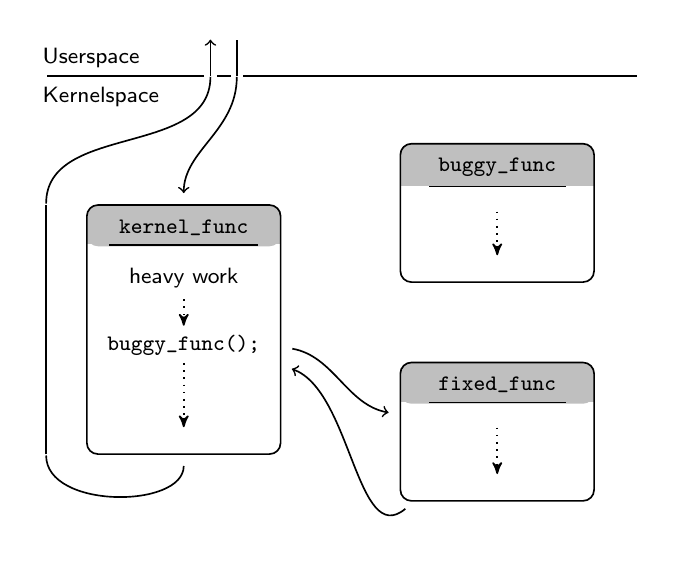
\begin{tikzpicture}[node distance=6mm, font=\sffamily\footnotesize]
      %%%%%%%%%%%%%% kern_fun
      \node [visible on=<1->, ent, minimum height=90pt] (WHOLE1) {};

      \node [visible on=<1->] (FNAME1) [below=2pt of WHOLE1.north] {\code{kernel_func}};
      \path [visible on=<1->, semithick] (FNAME1.south east) edge (FNAME1.south west);
      \begin{pgfonlayer}{background}
	\node [visible on=<1->, filltop] (TOPGRa1) [below=0pt of WHOLE1.north] {};
	\node [visible on=<1->, fillbot] (TOPGRb1) [above=0pt of FNAME1.south] {};
      \end{pgfonlayer}

      \node [visible on=<1->] (INSNa1) [below=5pt of FNAME1] { heavy work };

      \node [visible on=<1->] (INSNb1) [below=10pt of INSNa1] { \code{buggy_func();} }
        edge[visible on=<1->, codearrow, <-, shorten < = 0pt, shorten > = 0pt] node {} (INSNa1);

      \node (ARROW_START1) [below=-8pt of INSNb1] {}
	edge[visible on=<1->, codearrow] node {} (WHOLE1.south);

      %%%%%%%%%%%%%% buggy
      \node [visible on=<1->, ent, minimum height=50pt] (WHOLE2) [above right= -1cm and 1.5cm of WHOLE1] {};

      \node [visible on=<1->] (FNAME2) [below=2pt of WHOLE2.north] {\code{buggy_func}};
      \path [visible on=<1->, semithick] (FNAME2.south east) edge (FNAME2.south west);
      \begin{pgfonlayer}{background}
	\node [visible on=<1->, filltop] (TOPGRa2) [below=0pt of WHOLE2.north] {};
	\node [visible on=<1->, fillbot] (TOPGRb2) [above=0pt of FNAME2.south] {};
      \end{pgfonlayer}

      \node (ARROW_START2) [below=2pt of FNAME2] {}
	edge[visible on=<1->, codearrow] node {} (WHOLE2.south);

      %%%%%%%%%%%%%% fixed
      \node [visible on=<1->, ent, minimum height=50pt] (WHOLE3) [below=1cm of WHOLE2] {};

      \node [visible on=<1->] (FNAME3) [below=2pt of WHOLE3.north] {\code{fixed_func}};
      \path [visible on=<1->, semithick] (FNAME3.south east) edge (FNAME3.south west);
      \begin{pgfonlayer}{background}
	\node [visible on=<1->, filltop] (TOPGRa3) [below=0pt of WHOLE3.north] {};
	\node [visible on=<1->, fillbot] (TOPGRb3) [above=0pt of FNAME3.south] {};
      \end{pgfonlayer}

      \node (ARROW_START3) [below=2pt of FNAME3] {}
	edge[visible on=<1->, codearrow] node {} (WHOLE3.south);

      %%%%%%%%%%%%%% arrows
      \path [visible on=<2->, connarr, out=350, in = 170] (WHOLE1) edge (WHOLE3);
      \path [visible on=<2->, connarr, out=220, in = 340] (WHOLE3) edge (WHOLE1);

      %%%%%%%%%%%%%% KS/US
      \node (KSUS1) [above left=15mm and 5mm of WHOLE1] {};
      \node (KSUS2) [right=2cm of KSUS1] {}
        edge [thick] node {} (KSUS1);
      \node (KSUS3) [right=-5pt of KSUS2, inner sep=0pt, minimum size=0pt] {};
      \node (KSUS4) [right=-5pt of KSUS3] {};
      \node (KSUS5) [right=5pt of KSUS4] {}
        edge [thick] node {} (KSUS4);
      \node (KSUS6) [right=-5pt of KSUS5, inner sep=0pt, minimum size=0pt] {};
      \node (KSUS7) [right=-5pt of KSUS6] {};
      \node (KSUS8) [right=5cm of KSUS7] {}
        edge [thick] node {} (KSUS7);

      \node (US) [above right=-4pt and -5pt of KSUS1] {Userspace};
      \node (KS) [below right=-3pt and -5pt of KSUS1] {Kernelspace};

      \node (WHOLE1top) [above=of WHOLE1, minimum size = 0pt, inner sep=0pt] {};

      \node (WHOLE1bot) [minimum size = 0pt, inner sep=0pt, left=5mm of WHOLE1.south west] {};
      \node (WHOLE1bot2) [minimum size = 0pt, inner sep=0pt, left=5mm of WHOLE1.north west] {};

      \path [connarr, -, shorten > = 0pt, in=270, out=270] (WHOLE1.south) edge (WHOLE1bot);
      \path [connarr, -, shorten > = 0pt, shorten < = 0pt] (WHOLE1bot) edge (WHOLE1bot2);

      \path [connarr, -, shorten > = 0pt, shorten < = 0pt, in=270, out=90] (WHOLE1bot2) edge (KSUS3);
      \path [connarr, shorten < = 0pt, in=90, out=270] (KSUS6) edge (WHOLE1);

      \node (USEND1) [minimum size = 0pt, inner sep = 0pt, above=of KSUS3] {};
      \node (USEND2) [minimum size = 0pt, inner sep = 0pt, above=of KSUS6] {};

      \path [connarr, shorten < = 0pt] (KSUS3) edge (USEND1);
      \path [connarr, -, shorten < = 0pt] (KSUS6) edge (USEND2);

    \end{tikzpicture}
  \end{center}

\end{frame}

\begin{frame}
  \frametitle{Get It}

  \begin{itemize}
    \item Upstreaming
    \begin{itemize}
      \item \kgr was submitted and reviewed upstream
    \end{itemize}

    \pause

    \item There are other groups working on competing technologies
    \begin{itemize}
      \item \textsc{kPatch}, \textsc{kSplice}, criu-based aproach, \dots
      \item SUSE will work together with them
      \item Expectations: common standard kernel live patching
    \end{itemize}

    \pause

    \item Publishing
    \begin{itemize}
      \item Part of SLE12 kernel tree
      \item GIT repository upstream
      \begin{itemize}
	\item \url{http://git.kernel.org/pub/scm/linux/kernel/git/jirislaby/kgraft.git}
      \end{itemize}
    \end{itemize}
  \end{itemize}

\end{frame}

\begin{frame}
  \frametitle{Maintenance}

  \begin{itemize}
    \item \kgr patch is an RPM package
    \item Once installed, always protected
  \end{itemize}

\end{frame}

\section{Live Demo}

\begin{frame}
  \frametitle{Live Demo}

  \begin{itemize}
    \item Kernel with a security vulnerability
    \item Exploit program
    \item kGraft patch
  \end{itemize}

\end{frame}

\section{Conclusion}

\begin{frame}
  \frametitle{Conclusion}

  \heading{SUSE provides}
  \begin{itemize}
    \item Demanded live Linux kernel patching
    \item Dubbed \kgr
  \end{itemize}

\end{frame}

\end{document}
